% Generated by render.py; edit preamble.tex, citations.json and obstructions.tikz
\documentclass[border=12pt]{standalone}
\def\pgfsysdriver{pgfsys-dvisvgm.def}
\usepackage[dvisvgm]{xcolor}
\usepackage{xeCJK}
\setCJKmainfont{HaranoAjiGothic-Regular.otf}[BoldFont=HaranoAjiGothic-Bold.otf]
\setCJKsansfont{HaranoAjiGothic-Regular.otf}[BoldFont=HaranoAjiGothic-Bold.otf]
\usepackage{amsmath,amssymb,tikz,lmodern}
\usetikzlibrary{arrows.meta,positioning,calc,fit,backgrounds}
\renewcommand{\familydefault}{\sfdefault}
\definecolor{ink}{HTML}{25322F}
\definecolor{green}{HTML}{246657}
\definecolor{tint}{HTML}{EEF4F0}
\definecolor{soft}{HTML}{C6D2CC}
\definecolor{muted}{HTML}{52615B}
\newif\ifJapanese
\newcommand{\Tx}[2]{\ifJapanese #1\else #2\fi}
\newcommand{\Eff}{\overline{\operatorname{Eff}}}
\newcommand{\heading}[3]{{\color{green}\bfseries #1\quad\Tx{#2}{#3}}\\[5pt]}
% A white rectangle makes the complete citation label clickable, including spaces.
\newcommand{\refurl}[2]{\special{dvisvgm:raw <a xlink:href="#1" target="_blank" rel="noopener noreferrer">}{\setlength{\fboxsep}{0pt}\colorbox{white}{\color{green}\underline{\strut #2}}}\special{dvisvgm:raw </a>}}
\tikzset{
 card/.style={draw=soft,fill=white,rounded corners=2pt,align=left,text=ink,font=\fontsize{10.5}{14}\selectfont,inner xsep=12pt,inner ysep=10pt,text width=14.4cm},
 half/.style={card,text width=6.45cm,minimum height=2.05cm},
 result/.style={card,draw=green,fill=tint,line width=.9pt},
 reason/.style={align=left,text=muted,font=\fontsize{9}{12}\selectfont,inner sep=0pt,text width=12.6cm},
 branchreason/.style={reason,text width=5.95cm},
 edge/.style={-{Stealth[length=2.4mm]},draw=green,line width=1pt},
 wire/.style={draw=green,line width=1pt},
}
% Keep the arrow in a dedicated left gutter; explanations never cover it.
\def\flow#1#2#3;{
 \coordinate (#2-from) at ($(#1.south)+(-6.9,0)$);
 \coordinate (#2-to) at ($(#2.north)+(-6.9,0)$);
 \draw[edge] (#2-from)--(#2-to);
 \node[reason,anchor=west] (#2-reason) at ($(#2-from)!.5!(#2-to)+(.55,0)$) {#3};
}

% Style adapted from the repository's Schnell diagrams; MIT attribution retained.

% Generated from citations.json; do not edit.
\newcommand{\Cite}[1]{\csname cite-#1\endcsname}
\expandafter\def\csname cite-catalog\endcsname{\shortstack[l]{\refurl{https://github.com/openai/math/blob/1581d4cbdd69a0faf34b2089614fe2a814316a6a/overview.pdf}{OpenAI Research Catalog · Catalogue 046 · p. 6}}}
\expandafter\def\csname cite-fourfold\endcsname{\shortstack[l]{\refurl{https://github.com/openai/math/blob/1581d4cbdd69a0faf34b2089614fe2a814316a6a/preprints/A-projective-fourfold-with-large-fundamental-group-and-non-Stein-universal-cover-October-5-2026/large-fundamental-group-non-stein.pdf}{[OpenAI26a, Theorem 1.1, p. 1]}}}
\expandafter\def\csname cite-stein-obstruction\endcsname{\shortstack[l]{\refurl{https://github.com/openai/math/blob/1581d4cbdd69a0faf34b2089614fe2a814316a6a/preprints/A-projective-fourfold-with-large-fundamental-group-and-non-Stein-universal-cover-October-5-2026/large-fundamental-group-non-stein.pdf}{[OpenAI26a, Proposition 2.1, proof, p. 6]}}}
\expandafter\def\csname cite-remmert\endcsname{\shortstack[l]{\refurl{https://github.com/openai/math/blob/1581d4cbdd69a0faf34b2089614fe2a814316a6a/preprints/A-projective-fourfold-with-large-fundamental-group-and-non-Stein-universal-cover-October-5-2026/large-fundamental-group-non-stein.pdf}{[OpenAI26a, Section 1.1, p. 2]}}}
\expandafter\def\csname cite-surface\endcsname{\shortstack[l]{\refurl{https://github.com/openai/math/blob/1581d4cbdd69a0faf34b2089614fe2a814316a6a/preprints/A-surface-counterexample-to-Shafarevich-holomorphic-convexity-September-23-2026/paper.pdf}{[OpenAI26b, Theorem 1.1, p. 2]}}}
\expandafter\def\csname cite-hull\endcsname{\shortstack[l]{\refurl{https://github.com/openai/math/blob/1581d4cbdd69a0faf34b2089614fe2a814316a6a/preprints/A-surface-counterexample-to-Shafarevich-holomorphic-convexity-September-23-2026/paper.pdf}{[OpenAI26b, Lemma 1.2, pp. 4–5]}}}

\Japanesefalse
\begin{document}
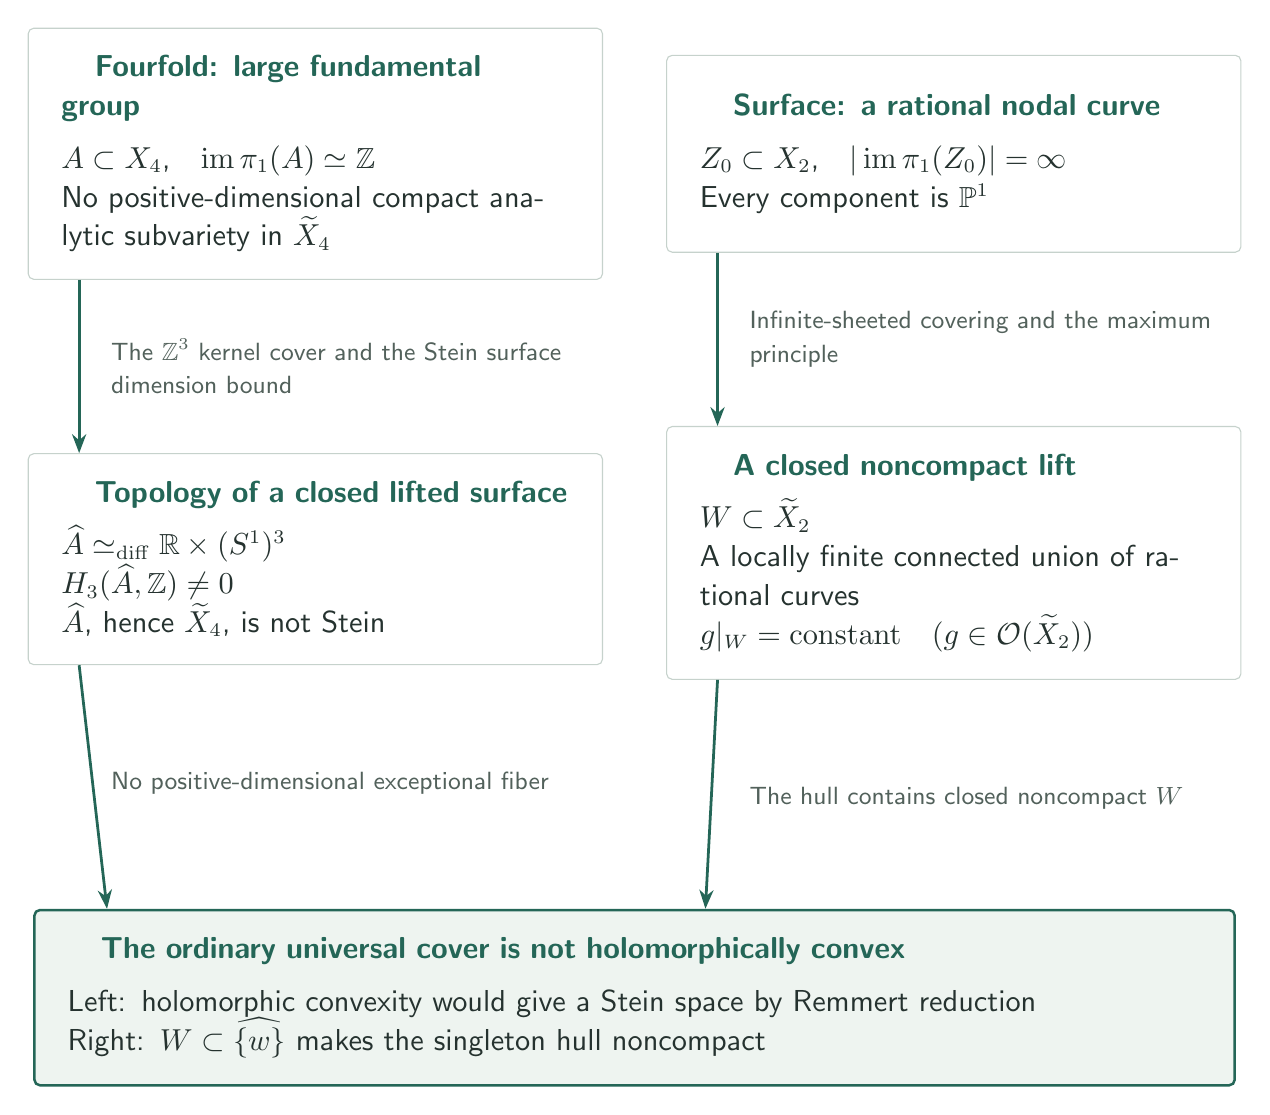
\begin{tikzpicture}
\node[half,minimum height=2.5cm] (a) {\heading{}{四次元：largeな基本群}{Fourfold: large fundamental group}
$A\subset X_4$,\quad $\operatorname{im}\pi_1(A)\simeq\mathbb Z$\\
\Tx{$\widetilde X_4$に正次元コンパクト解析部分多様体なし}{No positive-dimensional compact analytic subvariety in $\widetilde X_4$}};
\node[half,right=.8cm of a,minimum height=2.5cm] (b) {\heading{}{曲面：有理成分の曲線}{Surface: a rational nodal curve}
$Z_0\subset X_2$,\quad $|\operatorname{im}\pi_1(Z_0)|=\infty$\\
\Tx{各成分は $\mathbb P^1$}{Every component is $\mathbb P^1$}};
\node[half,below=2.2cm of a,minimum height=2.4cm] (c) {\heading{}{閉じた持上げ曲面の位相}{Topology of a closed lifted surface}
$\widehat A\simeq_{\rm diff}\mathbb R\times(S^1)^3$\\
$H_3(\widehat A,\mathbb Z)\ne0$\\
\Tx{$\widehat A$、したがって $\widetilde X_4$ は非Stein}{$\widehat A$, hence $\widetilde X_4$, is not Stein}};
\node[half,below=2.2cm of b,minimum height=2.4cm] (d) {\heading{}{閉・非コンパクトな持上げ}{A closed noncompact lift}
$W\subset\widetilde X_2$\\
\Tx{有理曲線の局所有限な連結和}{A locally finite connected union of rational curves}\\
$g|_W=\mathrm{constant}\quad(g\in\mathcal O(\widetilde X_2))$};
\draw[edge] ($(a.south)+(-3,0)$)--($(c.north)+(-3,0)$);
\node[branchreason,anchor=west] at ($(a.south)!.5!(c.north)+(-2.6,0)$) {\Tx{核 $\mathbb Z^3$ の被覆とStein曲面の次元制約}{The $\mathbb Z^3$ kernel cover and the Stein surface dimension bound}\\\Cite{stein-obstruction}};
\draw[edge] ($(b.south)+(-3,0)$)--($(d.north)+(-3,0)$);
\node[branchreason,anchor=west] at ($(b.south)!.5!(d.north)+(-2.6,0)$) {\Tx{無限枚被覆と最大値原理}{Infinite-sheeted covering and the maximum principle}\\\Cite{hull}};
\node[result,below=3cm of $(c.south)!.5!(d.south)$,anchor=north] (e) {\heading{}{通常の普遍被覆は正則凸でない}{The ordinary universal cover is not holomorphically convex}
\Tx{左：正則凸ならRemmert reductionが同型となりStein}{Left: holomorphic convexity would give a Stein space by Remmert reduction}\\
\Tx{右：$W\subset\widehat{\{w\}}$ により一点の正則包が非コンパクト}{Right: $W\subset\widehat{\{w\}}$ makes the singleton hull noncompact}};
\draw[edge] ($(c.south)+(-3,0)$)--($(e.north)+(-6.7,0)$);
\node[branchreason,anchor=west] at ($(c.south)+( -2.6,-1.5)$) {\Tx{正次元の例外ファイバーがない}{No positive-dimensional exceptional fiber}\\\Cite{remmert}};
\draw[edge] ($(d.south)+(-3,0)$)--($(e.north)+(.9,0)$);
\node[branchreason,anchor=west] at ($(d.south)+(-2.6,-1.5)$) {\Tx{閉・非コンパクトな $W$ が正則包に入る}{The hull contains closed noncompact $W$}\\\Cite{hull}};

\end{tikzpicture}
\end{document}
